\TODO{Motivation}

\subsection{Random grid search algorithm}\label{sswwupgrade:opt_rgs}
The chosen algorithm for optimizing the event selection is known as the Random Grid Search (RGS) \cite{2018.rgs-paper}.
Consider a simple case of two variables $x$ and $y$ chosen to differentiate the signal from the background.
In order to be considered a signal event, a given event would be required to pass a \emph{cut point} $\{x > x_c, y > y_c\}$.
A simple method to choose the optimal cut point (i.e. the ``best'' values of the cuts $x_c$ and $y_c$) would be to construct an $n\times m$ rectangular grid in $x$ and $y$ consisting of points $(x_0,y_0), (x_1,y_1), ..., (x_n,y_m)$, as in Figure~\ref{fig:rgs_square_grid}.
One can then choose a cut point $\{x > x_i, y > y_j\}$ that maximizes the signal significance as measured by a chosen metric.
This would be considered a \emph{regular} or \emph{rectangular} grid search.

While effective, this rectangular grid search comes with two major drawbacks:
\begin{enumerate}
\item The algorithm does not scale well as the number of variables to be optimized (i.e. the dimensionality of the grid) increases.  In the case of a square grid with $N$ bins per dimension $d$, the number of cut points to be evaluated grows as $N^d$.
\item Signal and background samples are rarely evenly distributed over the entire grid, resulting in many cut points being sub-optimal and evaluating them would be a waste of computing resources.
\end{enumerate}

To combat these problems, the RGS algorithm constructs a grid of cut points directly from the signal sample itself.

\begin{figure}[htp]
  \centering
  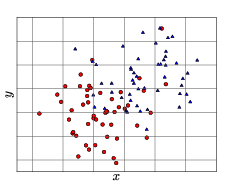
\includegraphics[width=0.48\textwidth]{figs/ssww_upgrade/rgs/figures_cuts_regulargrid}
  \caption{\TODO{replace with own figure}}   
  \label{fig:rgs_square_grid}
\end{figure}

\subsection{Inputs to the optimization}\label{sswwupgrade:opt_inputs}

\subsection{Results of the optimization}\label{sswwupgrade:opt_results}
